\documentclass[10pt]{article}
\usepackage[utf8]{inputenc}
\usepackage[shortlabels]{enumitem}
\usepackage[margin=1in]{geometry}
\usepackage{setspace}
\usepackage{hyperref}
\usepackage{graphicx}
\usepackage{natbib}
\onehalfspacing
\setlength{\parskip}{1em}
\setlength{\parindent}{0pt}
\bibliographystyle{ecta}
\usepackage[T1]{fontenc}
\usepackage{titling}
\usepackage{amsmath}
\setlength{\droptitle}{-7em}
\addtolength\abovedisplayskip{-3in}
\addtolength\belowdisplayskip{-3in}

\title{City Location Choice and Household Productivity}
\preauthor{}
\postauthor{}
\author{Tan Sein Jone}
\predate{}
\postdate{}
\date{}
%\Today

\begin{document}
\doublespacing
\maketitle

\section{Introduction}

Cities capture a disproportionate amount of household location choices in the world. In 2018, 55\% of the world's population lived in urban areas, and this is expected to increase to 68\% by 2050. This is because of the benefits cities provide, such as access to jobs, amenities, and social networks. These benefits are often thought of as universal to all households, regardless of their occupation specific skills. However, the benefits of every city is clearly not the same for every household. An auto worker from Detroit will not view New York as an equivalent substitute for a city to live in as a finance worker from New York. Given the billions of dollars spent on place based policies, it is important for us to separate out this dimension of comparative advantage, where a city is able to provide higher levels of productivity for households working in specific occupations.

A city's comparative advantage exists in three dimensions. First, there is a city specific advantage which makes all occupations more productive in that city. This is due to the city's size, more specifically it's population which results in better amenities, more jobs, and a larger social network. Second, there is an occupation specific advantage which is universal across all cities. Some jobs are simply more productive than others and cities that specialize in that job will be observed as having a nigher overall choice shares of households. Think cities that specialize in highly attractive occupations such as professional services. Finally, there is a city-occupation specific advantage. A city with a comparative advantage in this dimension may have specific policies that make it more attractive for a specific occupation such as tax breaks for mechanics in Chicago. One crucial distinction we need to make is between occupations and sectors. Sectors are broad categories of jobs such as manufacturing, services, and agriculture. Occupations are specific jobs such as mechanic and clerk. Cities can specialize in occupations by specializing in sectors that most intensely use that occupation.

In this paper, we propose a model of city location choices based on a class of models in the quantitative trade literature first proposed by \cite{ek}. These models treat productivity as random draws from Fr\'{e}chet distributions, allowing for a non zero production of goods which will help us to account for small cities. \cite{redding} applies this model to an urban setting by loading city heterogeneity onto amenities, capturing the first dimension of comparative advantage. Both these models however rely on the independence assumption which treats that goods and cities are perfect substitutes for each other. \cite{lindandramondo} break this assumption by introducing a nested CES utility structure which allows for correlated draws of productivity within nests across countries. We will apply this structure to the urban setting by treating occupations as independent nests. This will allow us to capture substitution patterns where cities that have a similar occupational structure will be treated as better substitutes for each other. By doing this, we are able to capture the second and third dimensions of comparative advantage.

We start in the first section by adapting the model of \cite{lindandramondo} to the urban setting. Unlike their original paper where the nests are implied, we will explicitly model the nests as occupations. A few implications will result from this specification. First, we will be able to observe both overall city shares and city shares specific specific to each occupation. As well as city occupation compositions which can be used as a measure of similarity between cities. Second, using this data, we will derive elasticities for all three dimensions of comparative advantage, that being the city specific, occupation specific and city-occupation specific elasticities. While the last elasticity will serve as a sanity check for the direction of substitution. City and occupation elasticities will be used to verify our claim of unbalanced substitution patterns that favor similar cities. In other words, shocks to cities of a certain occupational composition will have larger effects of cities with similar compositions due to correlations in productivity draws.

In the second section, we will be presenting our estimation strategy, exploiting variation over time to recover recover two important parameters of our model, that being the correlation parameter $\rho$ and the shape parameter $\theta$, which as we will discuss later on, determines the within and across occupation migration patterns. In the process, we will also recover our city, occupation and city-occupation specific shifters.

We will then take these estimation equations to data in the third section, using data from the American Community Survey which has on the metropolitan area and occupational level. We will start off by presenting some stylized facts about cities and their compositions to compare how similar the top cities are. This fully calibrated model will then be used to run counterfactual analysis and simulate the effects of a policy at both the city and occupation level. This is where it is possible for us to evaluate the effectiveness of place based policies and also where we will make statements about how these policies should be designed to maximize their effectiveness.

\section{Model}

\begin{align*}
    Y_{ck} = Z_{ck}
\end{align*}

Consider a closed economy consisting of $N$ cities and $K$ occupations. Each city $c$ employs households in occupation $k$ to produce output $Y_{ck}$. We assume no trade costs between cities and that the price of the good produced is freely traded and priced under perfect competition. The price index of city $c$ is given by $\Phi_c$ and the wage of a household living in city $c$ working in occupation $k$ is given by $w_{ck} = \Phi_c Z_{ck}$ where $Z_{ck}$ is the productivity of the household. We assume that when a household chooses to work in a particular occupation, they will be randomly allocated to a sector within a given city. A household has symmetric CES preferences over cities and occupations and will choose a city-occupation pair that maximizes their utility. We will assume that households are perfectly mobile across cities and that there are no fixed costs to moving. The productivity of a household within a given city-occupation is drawn from a Fr\'{e}chet distribution. In \cite{ek}, the Fr\'{e}chet distribution is used to model productivity draws in a trade setting and has two main components. The shape parameter $\theta$ which determines the dispersion of draws across the distribution and reflects the heterogeneity of cities. $\theta$ will also determine the gains from city choices, ie how much households will gain from having more choices of cities to live in, which is analogous to gains from trade. The scale parameter $T_{ck}$ is a level shifter that determines the absolute advantage of a city-occupation pair, reflecting its attractiveness. Our specification so far assumes independent draws of productivity across cities, the joint distribution of which is given by:

\begin{align*}
    P[Z_1 < z_1, \dots, Z_N < z_N] & = \prod_{c}^{N} P[Z_c < z_c]                                 \\
                                   & = \exp \left\{ - \sum_{c}^{N} T_{ck} Z_c^{- \theta} \right\}
\end{align*}

This result implies that the choice shares of households for a given city is equal to the probability of households choosing that city. So far, we have stuck with the the base EK specification with the only modification being the mapping of productivity onto wages rather than prices which allows us to obtain city choice shares. We will now abandon the independence assumption and introduce a structure that allows for correlated draws across cities.

\begin{align*}
    P[Z_1 < z_1, \dots, Z_N < z_N] = \exp \left\{ - \left( \sum_{c}^{N} (T_{ck} Z_c^{- \theta})^{\frac{1}{1 - \rho}} \right)^{1 - \rho} \right\}
\end{align*}

Notice with this structure that the shape of the distribution is no longer purely determined by $\theta$ but also by the correlation parameter $\rho$. Where the distribution of productivity within a given occupation decreases as $\rho$ increases. Meaning that within a given occupation, the higher correlation will result in cities being more similar with each other in terms of productivity. When $\rho = 0$, the distribution reduces down to the original joint distribution with the shape being purely determined by $\theta$ and where draws are independent. As $\rho \rightarrow 1$, the draws become perfectly correlated and the productivity is identical across all cities.

\subsection{Cross Nested CES}

\begin{align}
    P[Z_1(\nu) < z, \dots, Z_N(\nu) < z] = \exp \left\{ - \sum_{k}^{K} \left[ \sum_{c}^{N} (T_{ck} Z_c^{- \theta})^{\frac{1}{1 - \rho_k}} \right]^{1 - \rho_k} \right\}
\end{align}

We will assume that productivity is distributed max stable multivariate Fr\'{e}chet with $T_{ck}$ being the scale parameter for city $c$ and occupation $k$. $\theta > 0$ is the shape parameter that determines the dispersion of draws across the distribution and $\rho_k$ is the occupation specific correlation parameter. As in \cite{lindandramondo}, we adopt a cross nested CES structure with a correlational structure within independent occupational nests. This has the characteristic of distributions not purely determined by $\theta$ but also by the correlation parameter. This is because the correlation parameter determines the degree of correlation between draws of productivity across cities.

In order to identify the three dimensions of comparative advantage, we will be separating out the scale parameter into three components where $T_{ck} = T_c T_k t_{ck}$. $T_c$ is the city specific scale parameter which captures the attractiveness of a city, shifting the distribution of all productivity draws within that city upwards. $T_k$ is the occupation specific scale parameter which is common across all cities, this captures the effect that any occupation has across all cities. $t_{ck}$ is the city-occupation specific scale parameter which captures the effect of a city on a specific occupation. This will give us the final dimension of comparative advantage.

\begin{align}
    Z = \max_c \left\{ \frac{Z_c}{\Phi_c} \right\}
\end{align}

A household's schedule of productivity is characterized by a vector of draws from different Fr\'{e}chet distributions for each city occupation pair. The realized productivity a household has in city $c$ is the occupation that maximizes the productivity has in the city. Unlike sequential games where households might pick a city before picking an occupation, we assume that households pick both simultaneously. A way to contextualize this is to think of households as already having an ideal occupation in mind when picking a city, hence $Z_c = \max_k \left\{ Z_{ck} \right\}$. This productivity is then scaled by the price index of a city to reflect how high prices reduces the purchasing power of the household within that city, hence making it less attractive.

\subsection{Equilibrium}

\begin{align}
    G(Z_1^{- \theta}, \dots, Z_N^{- \theta}) = \sum_{k}^{K} T_k \left[ \sum_{c}^{N} (t_{ck} Z_c^{- \theta})^{\frac{1}{1 - \rho_k}} \right]^{1 - \rho_k}
    \label{nested_ces}
\end{align}

We first define $Z_c^{- \theta} = (\gamma w_c)^{- \theta} T_c$ and $\gamma = \Gamma (\frac{\theta + 1 - \rho_k}{\theta})^{\frac{1}{1 - \rho_k}}$. Given our definition of $Z_c^{- \theta}$, $T_c$ will be absorbed within $Z_c^{- \theta}$, giving us the correlation function $G(Z_1^{- \theta}, \dots, Z_N^{- \theta})$ as defined in equation \ref{nested_ces}.

\begin{align*}
    \pi_c = \frac{Z_c^{- \theta} G_c(Z_1^{- \theta}, \dots, Z_N^{- \theta})}{G(Z_1^{- \theta}, \dots, Z_N^{- \theta})}
\end{align*}

Where $G_c (Z_1^{- \theta}, \dots, Z_N^{- \theta}) = \partial G(Z_1^{- \theta}, \dots, Z_N^{- \theta}) / \partial Z_c^{- \theta}$. The expression above gives us the city specific choice shares of households across all occupations. In order to evaluate the expression, we make the simplifying assumption that the correlation parameter is the same across all occupations $\rho_k = \rho$.

\begin{align*}
    \lambda_{k} = \sum_{c}^{N} \left( t_{ck} Z_{c}^{-\theta} \right)^{\frac{1}{1-\rho}}
\end{align*}

We introduce the above expression which measures the appeal of occupation $k$. Given that the expression does not include $T_k$, it does not capture the attractiveness of occupation $k$. Instead the expression captures the extent to which a given occupation $k$ exhibits city-specific productivities which are correlated with aggregate city-level attractiveness. The following definitions will be useful in simplifying the expression for city shares.

\begin{align*}
    \pi_{ck} = \frac{Z_c^{- \theta} G_c^k(Z_1^{- \theta}, \dots, Z_N^{- \theta})}{G^k(Z_1^{- \theta}, \dots, Z_N^{- \theta})}
\end{align*}

To obtain occupation specific choice shares, we can evaluate the derivative for city shares at the occupation level. More specifically, rather than $G(Z_1^{- \theta}, \dots, Z_N^{- \theta})$, we will be evaluating $G^k(Z_1^{- \theta}, \dots, Z_N^{- \theta}) = \sum_{c}^{N} (t_{ck} Z_c^{- \theta})^{\frac{1}{1 - \rho_k}}$. This will give us the following:

\begin{align}
    \pi_{ck} = \frac{(t_{ck} Z_c^{-\theta})^{\frac{1}{1 - \rho}}}{\lambda_k}
    \label{city_occuaption_shares}
\end{align}

Moving forward, it will be convenient for us to provide the following definitions. First, we define $\phi_{ck}$ as the comparative advantage of city $c$ in occupation $k$. This can be interpreted as an occupation's within city choice shares. As such $\phi_{ck}$ will be between 0 and 1. We define this formally as:

\begin{align}
    \phi_{ck} \equiv \frac{{t^{\frac{1}{1-\rho}}_{ck}}{T_{k}}\lambda_{k}^{-\rho}}{\sum\limits_{k}{t^{\frac{1}{1-\rho}}_{ck}}{T_{k}}\lambda_{k}^{-\rho}}
    \label{occupation_by_city_shares}
\end{align}

Second, we define an occupation specific choice share which takes into account both the size of each occupation, as measured by productivity $T_k$, and the extent to which individual city-occupation productivities are correlated with overall city attractiveness. This is defined as the following expression:

\begin{align}
    \omega_k \equiv \frac{{T_{k}}\lambda_{k}^{1-\rho}}{\sum\limits_{k}{T_{k}}\lambda_{k}^{1-\rho}}
    \label{occupation_shares}
\end{align}

From the perspective of discrete choice demand models, $\omega_k$ can be interpreted as the "market share" of occupation $k$. This is because it captures the extent to which the productivity of occupation $k$ is correlated with overall city attractiveness. The expression is normalized by the sum of all $\omega_k$ to ensure that the sum of all market shares is equal to 1.

\begin{align}
    \frac{\pi_{ck}}{\pi_c}\equiv \frac{\phi_{ck}}{\omega_k}
    \label{identity}
\end{align}

The expression above tells us the extent to which a given occupation $k$ is concentrated in city $c$ above and beyond the predicted concentration, given the size of the city $\pi_c$ is equivalent to the within-city choice share in occupation $k$ divided by the aggregate choice share of that occupation.

\begin{align*}
    \pi_{c} = \sum_{k}^{K} \frac{(Z_{c}^{-\theta} t_{ck})^{\frac{1}{1-\rho}}}{\lambda_k} \frac{T_k \lambda_{k}^{1 - \rho}}{\sum \limits_{k}^{K} T_k \lambda_{k}^{1-\rho}}
\end{align*}

\begin{align}
    \pi_c = \sum_{k}^{K} \pi_{ck} \omega_k
\end{align}

By using our definitions, we arrive at the above expression for city shares, which is now the sum of all occupation specific shares weighted by the market share of each occupation.

\subsection{City-Occupation Elasticities}

We now turn to the city-occupation derivatives: city $c$'s own technology elasticity and cross technology elasticity with respect to another city $c'$. This derivative will be approximated by assuming that each city is small, and therefore $\partial \ln \lambda_k / \partial \ln t_{ck} \approx 0$. That is, the aggregate "price index" associated with location choice in occupation $k$ is not affected by a marginal change in the productivity of a given city-occupation pair. We then obtain the following for the own technology shock:

\begin{align}
    \frac{\partial \ln \pi_{ck}}{\partial \ln t_{ck}} \approx \phi_{ck} \left( \frac{1}{1 - \rho} \right)
    \label{co_own_elasticity}
\end{align}

This elasticity is positive and increasing in a city's comparative advantage in occupation $k$. The intuition is that a city that is more attractive for occupation $k$ will see a larger increase in the choice share of that occupation in response to a marginal increase in the productivity of that occupation. The more specialized the city is in that occupation, the larger the effect of a productivity shock in that occupation. As $\rho \rightarrow 1$, the elasticity approaches infinity, as within any given occupation, if they become more correlated, cities within that given occupation become perfect substitutes for each other.

\begin{align}
    \frac{\partial\ln{\pi_{c}}}{\partial\ln{t_{{c'}k}}} = -{\pi_{c'}}{\phi_{ck}}\Big[1+\Big(\frac{\rho}{1-\rho}\Big)\Big(\frac{\pi_{ck}}{\pi_{c}}\Big)\Big]
    \label{co_cross_elasticity}
\end{align}

Turning our attention to the cross city technology elasticity, we see that the first term captures the CES element of consumer choice. As the city $c'$ increases in size and becomes increasingly competitive in that occupation, any shocks to this city-occupation pair will have an increasingly negative effects on all other cities.

How much the other cities will be affected is captured by the second term which captures the unbalanced substitution patterns. If a city is relatively concentrated in occupation $k$, then the affects of a shock in that given occupation will be felt more severely, this is shown by the ratio $\pi_{ck} / \pi_c$. Notice also that if $\rho = 0$, this elasticity simplified to the standard CES elasticity. As $\rho \rightarrow 1$, the elasticity approaches infinity and the correlated choices start to dominate.

\subsection{Aggregate Elasticities}

We now consider the elasticity of city shares with respect to aggregate city technology shocks $T_c$ and aggregate occupation shocks $T_k$. Beginning with the former, if we assume again that each cit is small and that $\partial \ln \lambda_k / \partial \ln T_c \approx 0$, we get the following for a city's own technology shock:

\begin{align*}
    \frac{\partial \ln \pi_c}{\partial \ln T_c} \approx \frac{1}{1 - \rho}
\end{align*}

This is simply the summation of city-occupation elasticities which was derived in expression \ref{co_own_elasticity}. And given that by definition $\sum \limits_k^K \phi_{ck} = 1$, we get the following derivations:

\begin{align*}
    \frac{\partial{\ln{\pi_{c}}}}{\partial\ln{T_{c}}} & = \sum\limits_{k}\frac{\partial{\ln{\pi_{c}}}}{\partial\ln{t_{ck}}} \\ &= \sum\limits_{k}\phi_{ck}\Bigg(\frac{1}{1-\rho}\Bigg) \\ &= \Bigg(\frac{1}{1-\rho}\Bigg)\sum\limits_{k}\phi_{ck} = \frac{1}{1-\rho}
\end{align*}

The result tells us that if $\rho = 0$ and there's no correlation between occupations, then the elasticity is simply 1. We get a similar story when deriving the cross city technology elasticity. Using the same assumption, we arrive at the result:

\begin{align}
    \frac{\partial\ln{\pi_{c}}}{\partial\ln{T_{c'}}} = -\pi_{c'}\Bigg[\sum\limits_{k}\phi_{{c'}k}\Big[1+\Big(\frac{\rho}{1-\rho}\Big)\Big(\frac{\pi_{ck}}{\pi_{c}}\Big)\Big]\Bigg]
\end{align}

Similarly, this is simply the sum over all city-occupation elasticities derived in expression \ref{co_cross_elasticity}. This is shown in the following derivation:

\begin{align*}
    \frac{\partial\ln{\pi_{c}}}{\partial\ln{T_{c'}}} & = \sum\limits_{k}\frac{\partial\ln{\pi_{c}}}{\partial\ln{t_{{c'}k}}} \\ &= \sum\limits_{k}\Bigg[-{\pi_{c'}}{\phi_{ck}}\Big[1+\Big(\frac{\rho}{1-\rho}\Big)\Big(\frac{\pi_{ck}}{\pi_{c}}\Big)\Big]\Bigg]\\ &= -\pi_{c'}\Bigg[\sum\limits_{k}\phi_{{c'}k}\Big[1+\Big(\frac{\rho}{1-\rho}\Big)\Big(\frac{\pi_{ck}}{\pi_{c}}\Big)\Big]\Bigg]
\end{align*}

The interpretation of this elasticity is the same as expression \ref{co_cross_elasticity}. The first term captures the CES element of consumer choice and the second term captures the unbalanced substitution patterns, with $\rho$ governing the strength of this unbalanced substitution. Now we simply sum over all occupations to get the aggregate elasticities.

Lastly, we derive the elasticity of city shares with respect to aggregate occupation shocks $T_k$. This is fairly straightforward as wel can simply evaluate the following:

\begin{align*}
    \frac{\partial\ln{\pi_{c}}}{\partial\ln{T_{k}}} & = \Big(\frac{\partial{\phi_{ck}}}{\partial{T_{k}}}\Big)\Big(\frac{T_{k}}{\phi_{ck}}\Big) - \Big(\frac{\partial{\omega_{k}}}{\partial{T_{k}}}\Big)\Big(\frac{T_{k}}{\omega_{k}}\Big) \\ &= \phi_{ck}-\omega_{k}
\end{align*}

By using the identity in expression \ref{identity}, we can rewrite the elasticity as the following:

\begin{equation}
    \frac{\partial\ln{\pi_{c}}}{\partial\ln{T_{k}}} = {\omega_{k}}\Bigg[\frac{\pi_{ck}}{\pi_{c}}-1\Bigg]
\end{equation}

You should first notice that the second term in brackets can be either positive or negative depending on the city's relative concentration in that occupation. If the city is relatively concentrated and $\pi_{ck} / \pi_c > 1$, then the city will face a negative shock. If the city is relatively less concentrated and $\pi_{ck} / \pi_c < 1$, then the city will face a negative shock. We can think of this as certain occupations start to become more attractive, cities that are less concentrated in that occupation will face a negative shock as households start to move to cities that are more concentrated in that occupation. This second term is scaled by the market share of that occupation, $\omega_k$, which is simply the market share of that occupation across all cities.

\section{Estimation Strategy}

% \subsection{Shifters}

% Given our model, we have 4 sets of shares that we can consider. City shares $\pi_c$, city shares for each occupation $\pi_{ck}$, occupation market shares $\omega_k$ and occupation shares for each city $\phi_{ck}$. In order for us to recover city and city-occupation specific shifters, consider the following estimation equation derived from expression \ref{city_occuaption_shares}:

% \begin{align*}
%     \ln \pi_{ck} & = \frac{1}{1 - \rho} \ln t_{ck} - \frac{1}{1 - \rho} \ln Z_c^{- \theta} - \ln \lambda_k \\
%                  & = \hat{\epsilon_{ck}} + + \hat{\eta_c^1} + \hat{\delta_k^1}
% \end{align*}

% This will be a simple OLS regression with city and occupation level fixed effects on city shares by occupation. With $\hat{\eta_c^1}$ being our city specific shifter, $\hat{\delta_k^1}$ being our occupation specific shifter and $\hat{\epsilon_{ck}}$ being our residuals.

% \begin{align*}
%     t_{ck}         & = exp \left(  (1 - \rho) \hat{\epsilon_{ck}}\right)  \\
%     \lambda_k      & = exp \left( (1 - \rho) \hat{\eta_c^1} \right)       \\
%     Z_c^{- \theta} & = exp \left( - \hat{\delta_k^2 }\right)              \\
%     T_c            & = Z_c^{- \theta} \left( \gamma \Phi_c \right)^\theta
% \end{align*}

% The equations above allow us to recover our city and city-occupation specific scale parameters. $\lambda_k$ will be used shortly to recover our occupation specific scale parameters.

% \begin{align*}
%     \ln \phi_{ck} & = \frac{1}{1 - \rho} \ln t_{ck} + \ln T_k \lambda_k^{- \rho} - \ln \left( \sum_k^K t_{ck}^{\frac{1}{1 - \rho}} T_k \lambda_k^{- \rho} \right) \\
%                   & = \hat{\epsilon_{ck}} + \hat{\delta_k^2} + \hat{\eta_c^2}
% \end{align*}

% Similarly, we will be using our occupation shares defined in expression \ref{occupation_by_city_shares} and have it be regressed against city and occupation fixed effects. Given that we have already identified $\lambda_k$, we can use this to recover our occupation specific scale parameters which is given by the equation below:

% \begin{align*}
%     T_k = \lambda_k^\rho e^{\hat{\delta_k^2}}
% \end{align*}

\subsection{Within-Occupation Migration}

Notice that for us to estimate our shifters, we have to first recover our $\rho$ parameter. To do so, we exploit a variation in city-occupation shares over time. Consider the following equation at the city-occupation-year level. From expression \ref{city_occuaption_shares}, we can get the following:

\begin{align*}
    \ln \pi_{ck} & = \frac{1}{1 - \rho} \ln t_{ckt} - \frac{1}{1 - \rho} \ln Z_{ct}^{- \theta} - \ln \lambda_{kt}
\end{align*}

Now we assume the following relationship productivity and wages at the city-occupation level: $t_{ckt} = w_{ckt} \eta_{ckt}$. Where $w_{ckt}$ are pages paid and $\eta_{ckt}$ is productivity. This will give us the following model:

\begin{align*}
    \ln \pi_{ckt} = \left( \frac{1}{1 - \rho} \right) \ln w_{ckt} + \delta_{ct} + \delta_{kt} + \eta_{ckt}
\end{align*}

With some abuse of notation, we have defined $\eta_{ckt} = \ln \eta_{ckt}$. We now take differences over time to eliminate level shifts.

\begin{align*}
    \Delta_t \ln \pi_{ckt} = \left( \frac{1}{1 - \rho} \right) \Delta_t \ln w_{ckt} + \delta_{ct} + \delta_{kt} + \Delta_t \eta_{ckt}
\end{align*}

We can estimate this equation by regressing wages on city occupation shares and using city and occupation fixed effects at the city-occupation level for every year with $\delta_{ct}$ being city fixed effects and $\delta_{kt}$ being occupation fixed effects. Given that $\hat{\rho} \in (0, 1)$, we will end up with the restriction $\hat{\beta} \in [1, +\infty)$.

With this regression, we are testing whether migration decisions are primarily within occupations rather than across occupations. If the correlation parameter is close to 1, then migration decisions are purely within occupations. Notice that as $\hat{\rho}$ increases, $\hat{\beta}$ increases. From this perspective, we can interpret $\rho$ as governing within-occupation migration and $\theta$ as governing across-occupation migration.

\begin{align*}
    Y_{st} = A_{st} \prod_{k}^{K} Q_{kst}^{\gamma_{ks}}
\end{align*}

One concern with the initial specification is the endogeneity of wages with the error term,more explicitly $cov[w_{ckt}, \eta_{ckt}] \neq 0$. In order to instrument for the change in wages, we will use a shift share in which we make use of sectors. Here, we define a Cobb-Douglas strcture of production where the intensity of occupation $k$ in sector $s$ is given by $\gamma_{ks}$ such that $\sum_{k}^{K} \gamma_{ks} = 1$. We will use the shift share of occupation $k$ in sector $s$ as an instrument for the change in wages. $A_{st}$ will be the total factor productivity of sector $s$ in year $t$.

\begin{align*}
    w_{ckt}^{IV} = \sum_{s}^{S} \gamma_{ks} \kappa_{cs} A_{st}
\end{align*}

where $\kappa_{cs}$ is the  share of occupation $k$ in sector $s$ in city $c$. This will give us the following first stage regression:

\begin{align*}
    \ln w_{ckt}^{IV} = \beta^{IV} \ln w_{ckt}^{IV} + \delta_{ct} + \delta_{kt}^{IV} + \eta_{ckt}^{IV}
\end{align*}

We will then use the predicted values of $\ln w_{ckt}^{IV}$ as our instrument in the second stage regression.

\begin{align*}
    \ln \pi_{ckt} = \left( \frac{1}{1 - \rho} \right) \ln w_{ckt}^{IV} + \delta_{ct} + \delta_{kt} + \eta_{ckt}
\end{align*}

\subsection{Across Occupation Migration}

Given that we've identified $\rho$, we can now proceed to estimate our shape parameter $\theta$ and in the process recover all our scale parameters. We start with occupation market shares $\omega_k$ in expression \ref{occupation_shares}. By taking relative shares, we get the following:

\begin{align*}
    \frac{\omega_{kt}}{\omega_{k't}} = \frac{T_{kt} \lambda_{kt}^{1 - \rho}}{T_{k't} \lambda_{k't}^{1 - \rho}}
\end{align*}

Subject to normalization to some base occupation year, we can estimate $T_{kt} \lambda_{kt}^{1 - \rho} \forall (k, t)$. We can then use this to recover the denominator in $\omega_k$ and get $\sum_{k}^{K} T_{kt} \lambda_{kt}^{1 - \rho} \forall t$. This will be useful in recovering our city and city occupation specific scale parameters. Now consider the city-occupation shares from expression \ref{city_occuaption_shares} taken in logs and transformed into a form with fixed effects:

\begin{align*}
    \ln \pi_{ckt} & = \frac{1}{1 - \rho} \ln t_{ckt} - \frac{1}{1 - \rho} \ln Z_{ct}^{- \theta} - \ln \lambda_{kt} \\
                  & = \hat{\epsilon}_{ckt} + \hat{\delta}_{ct} + \hat{\delta}_{kt}
\end{align*}

such that,

\begin{align*}
    \hat{\lambda}_{kt} & = \exp \left( - \hat{\delta}_{kt} \right)             \\
    \hat{t}_{ckt}      & = \exp \left( (1 - \rho) \hat{\epsilon}_{ckt} \right) \\
\end{align*}

We can then use the estimated $\hat{\lambda}_{kt}$ to recover our occupation specific scale parameters:

\begin{align*}
    \hat{T}_{kt} = \frac{\widehat{\sum_{k}^{K} T_{kt} \lambda_{kt}^{1 - \rho}}}{\hat{\lambda}_{kt}^{1 - \rho}}
\end{align*}

Now we need some way for us to recover productivity in order to estimate the shape parameter $\theta$. Consider the following modification to city shares using our recovered parameters:

\begin{align*}
    \tilde{\pi}_{ct} & = \pi_{ct} \frac{\sum_{k}^{K} T_{kt} \lambda_{kt}^{- \rho}}{\sum_{k}^{K} t_{ckt}^{\frac{1}{1 - \rho}} T_{kt} \lambda_{kt}^{1 - \rho}} \\
                     & = Z_{ct}^{- \frac{\theta}{1 - \rho}}
\end{align*}

We now take logs and difference the equation to eliminate the level shift. Recalling our definition of $Z_c^{- \theta} = (\gamma w_c)^{- \theta} T_c$, we get the following estimation equation:

\begin{align*}
    \Delta_t \ln \hat{\pi}_{ct} = \hat{\beta} \Delta_t \ln w_{ct} + \Delta_t \hat{\eta}_{ct}
\end{align*}

The differencing will eliminate $\gamma$, which is constant over time, leaving us with a regression of changes in wages and city fixed effects over time on changes in city shares. The coefficient $\hat{\beta}$ will be our estimate of $ - \theta / (1 - \rho)$, which when rearranged gives us $\hat{\theta} = - \hat{\beta} (1 - \hat{\rho})$. Note the relationship between $\theta$ and $\rho$ is such that as $\rho$ increases, $\theta$ decreases. This indicates that as the strength of within occupation migration increases, the across occupation migration becomes less important, reinforcing our interpretation of $\rho$ as governing within-occupation migration and $\theta$ as governing across-occupation migration.

\begin{align*}
    \hat{T}_{ct} = exp \left( (1 - \rho) \hat{\eta}_{ct} \right)
\end{align*}

Using this regression, we also recover city level shifters from fixed effects estimates.

\section{Empirical Results}

\subsection{Data}

We will be using data from the American Community Survey (ACS) which is a survey conducted by the US Census Bureau. The ACS is a survey that collects data on the metropolitan area and occupational level. We will be using data from 2010 to 2022. The ACS provides data on the household level, detailing wages, metropolitan area, occupation and sector of employment based on NAICS codes. This will be used to construct our share data $\pi_c$ $\pi_{ck}$, $\omega_k$, $\phi_{ck}$ and $\phi_{cs}$ as well as obtain wage data $w_{ckt}$. We will also be using data from the Bureau of Labour Statistics to obtain total factor productivity data at the sector level $A_{st}$.

% \begin{figure}[!htb]
%     \centering
%     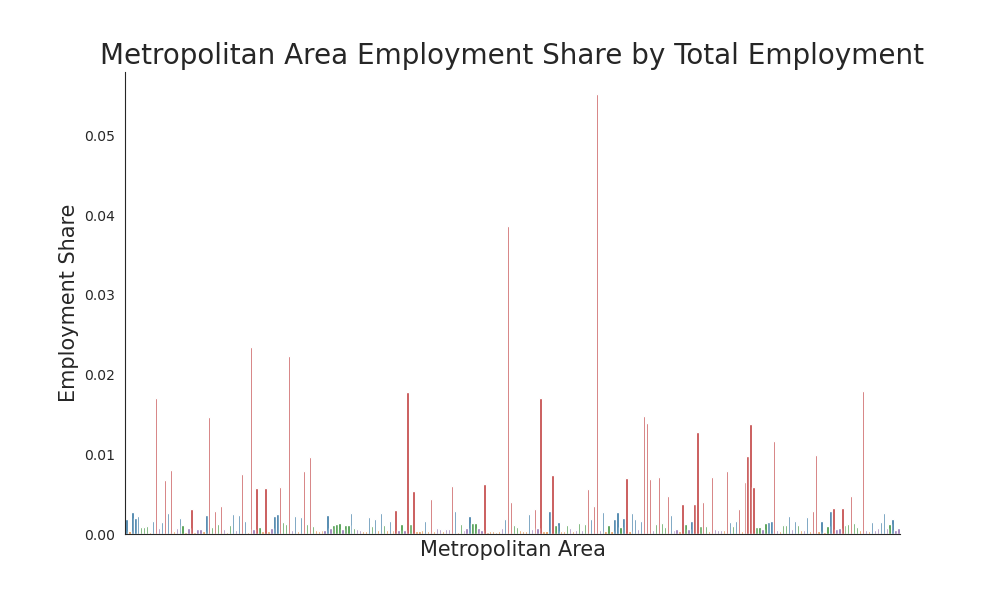
\includegraphics[width=\textwidth]{../../estimations/graphs/city_employment_share.png}
%     \caption{City Employment Share}
%     \label{employment_city_share}
% \end{figure}

% \begin{figure}[!htb]
%     \centering
%     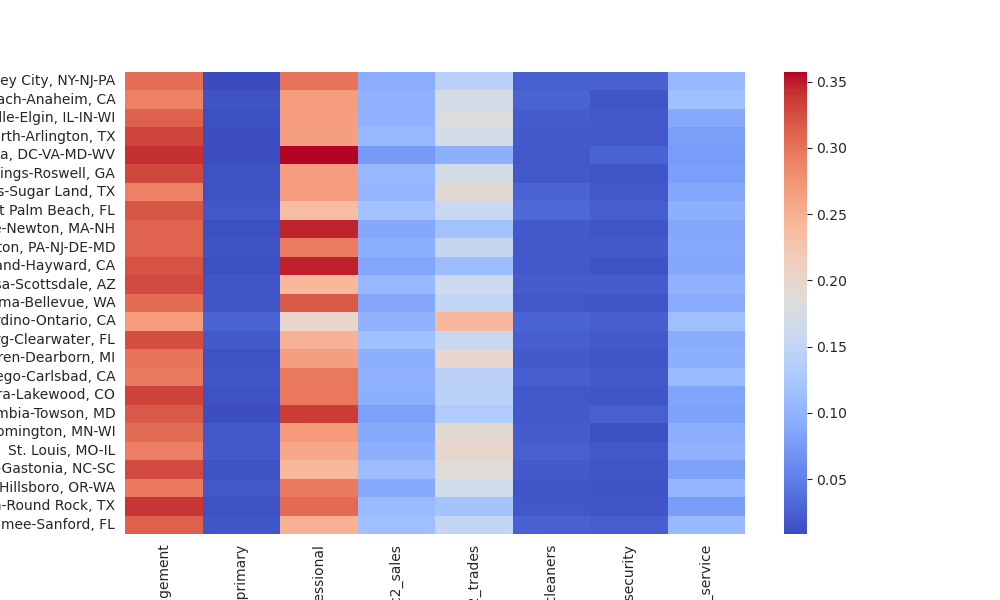
\includegraphics[width=\textwidth]{../../estimations/graphs/top_25_city_heatmap.png}
%     \caption{Occupation Shares by Cities}
%     \label{top_25_city_heatmap}
% \end{figure}

\begin{figure}[!htb]
    \centering
    \begin{minipage}{0.48\textwidth}
        \centering
        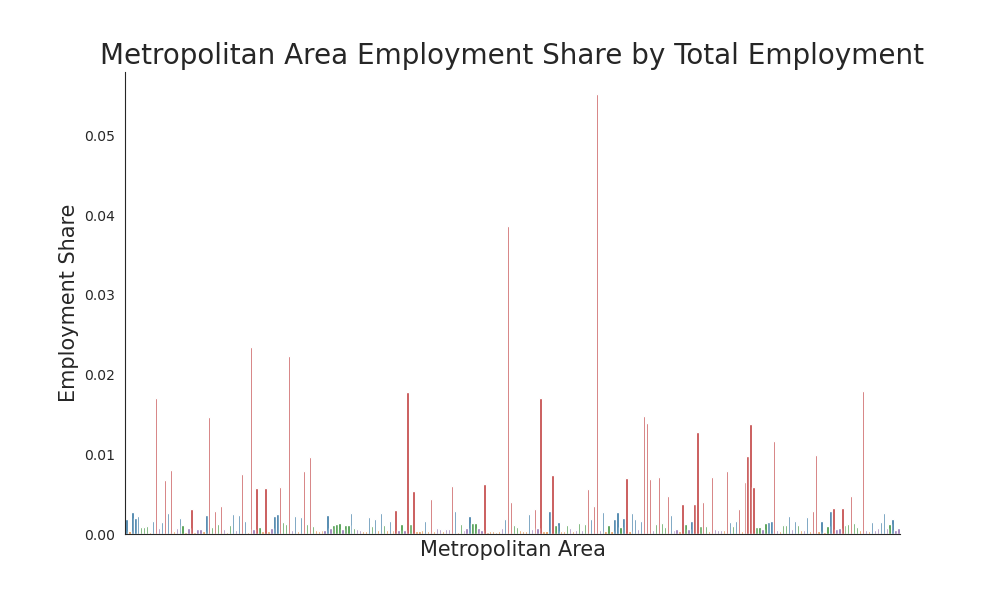
\includegraphics[width=\textwidth]{../../estimations/graphs/city_employment_share.png}
        \caption{City Employment Share}
        \label{employment_city_share}
    \end{minipage}\hfill
    \begin{minipage}{0.48\textwidth}
        \centering
        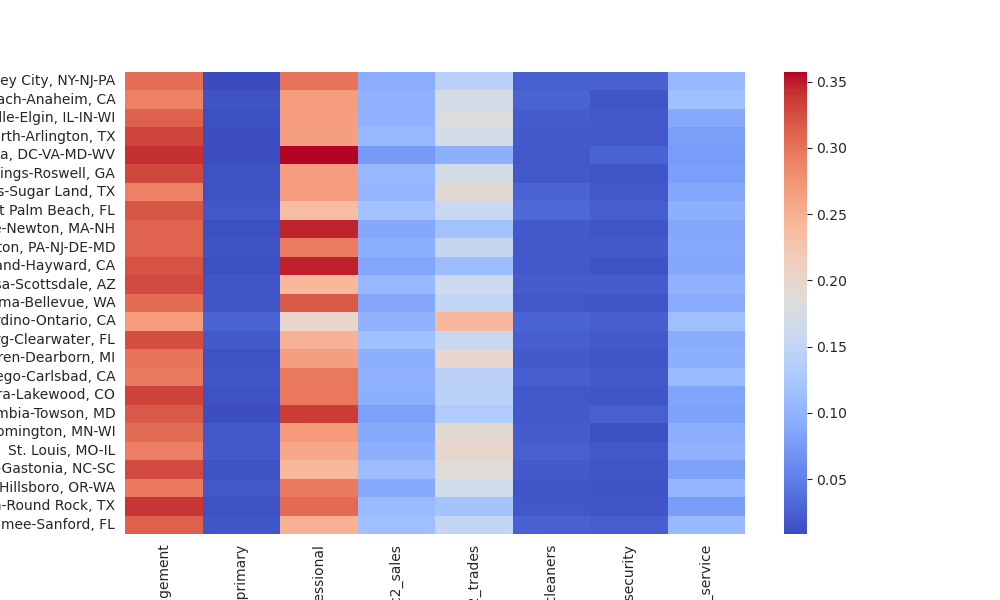
\includegraphics[width=\textwidth]{../../estimations/graphs/top_25_city_heatmap.png}
        \caption{Occupation Shares by Cities}
        \label{top_25_city_heatmap}
    \end{minipage}
\end{figure}

From the data in figure \ref{employment_city_share}, we see that a few metropolitan areas own a disproportionate share of employment which illustrates the size effects of cities to attract employment and households. Intuitively, we should expect these cities to be very different from each other in terms of their specialization, otherwise we would expect the largest city with a particular composition to dominate in the share of households. When zooming into the compositions of the top 25 cities however, we see a different story. In figure \ref{top_25_city_heatmap}, we see that the top 25 cities are very similar with each other in terms of their specialization. With all cities specializing in occupations like management and professional services. While there is some heterogeneity in the composition of cities, the specialization of cities is not as pronounced as we would expect. This indicates to us that the occupation shifter will play a large role in determining the attractiveness of a city.

\subsection{Results}

To recover our $\rho$ parameter, we run a two stage least squares regression with a shift share instrument. We find that this regression yields a high F-Statistic and a significantly higher estimate for $\hat{\beta}$ compared to ols. This ultimately results in a fairly high estimate of $\hat{\rho} = 0.67$. The result means that draws across cities within any given occupation id highly correlated and indicates to us that people are very likely to migrate within occupations. This is consistent with the idea that people are more likely to move to cities where they can find jobs in their occupation.

When taking a look at the regression of wages against city shares, we $\hat{\beta}$ to be fairly low, giving us a resulting $\theta$ of 0.02. This is surprising for a couple of reasons. First, it indicates to us that the shape of the Fr\'{e}chet distributions are mainly controlled by the correlation parameter $\rho$, meaning that across labor migration, meaning migration that is purely due to cities is not that important. Second, it means that migration is mainly within occupations rather than across occupations. Resulting in a dynamic where people are actually very willing to migrate, but only to cities that have the occupations they are looking for.

Given the previous result, we shouldn't be too surprised by the estimates of our shifters. In 2010, we find that occupation shifters are significantly higher compared to city shifters. This is reflective of our initial result indicating that occupations matter more to migration compared to cities themselves. For occupation shifters, what we find surprising is the significantly higher estimate of primary occupations, which suggests that these occupations are highly attractive to households. One interpretation that we can give is that since cities with primary occupations are likely small towns which tends to specialize in these occupations such as farming, while they are unattractive to any household who does not specialize in these occupations, they will be highly attractive to the ones who do. Meaning that since primary occupations can only be done in certain cities, households who specialize in these occupations will move to these cities even if the city itself is highly unattractive.

In contrast, for occupations that can be done in most cities and sometime even remotely like management and professional services, these occupations, while highly attractive in terms of salary, become less of a pull for households since these occupations can found in most cities. So for cities that specialize in these occupations, their elasticities will be higher compared to cities that specialize in primary occupations, which is consistent with the increase in migration between large cities. Unlike in the early 20th century where we observe a lot of rural urban migration, since most urban cities have started to develop similar compositions in terms of their occupations, we see people migrating between large cities due to people looking for the same occupations.

Unsurprisingly, the high estimates of occupation shifters mean that we obtain fairly low estimates of city shifters. The cities with the highest shifters are dense metropolitan areas such as New York and Los Angeles, reflecting the large population it attracts. Notable in our estimates is the variance in shifter estimates between cities, with some shifters being up to 3 times more than others, indicating significant heterogeneity in the attractiveness of cities. This makes sense as large cities tend to offer more and better amenities as well as better access to jobs, making them more attractive to households. We also find that city shifters tend to be fairly stable over time with changes being generally below 10\% over the 10 year period. Given how long it takes for cities to build infrastructure and other amenities in addition to needing to separate themselves from other cities, this is not surprising.

\section{Quantitative Exercises}

With our parameter and shifter estimates, we can now perform two counterfactual exercises. First, we will simulate a city specific shock in order to observe the patterns of migration across cities, more specifically, we will be interested in observing the unbalanced substitution patterns that favor similar cities. Second, we will examine what kinds of migration patterns result from a shock in a particular occupation. This will effectively simulate the effects of a trade shock which effect some occupations more than others. An example of this being the China shock.

\subsection{City Specific Shock}

Our results from the previous section suggest that while we may see some migration to large cities purely due to the size of the city, we should expect to see more migration to cities that have a similar occupational makeup. For this exercise, we will induce a negative shock of 50\% to all occupations in New York, which is a city that primarily has occupations in management and professional services. Taking a look at the results in Figure \textbf{placeholder}, we see that while there is some migration to cities purely due to their size, we find that the vast majority of people move to other similar cities such as Los Angeles and Chicago. This is consistent with our results that people are more likely to move to cities that have similar occupational compositions, reinforcing our argument that occupations matter more to migration compared to cities themselves. That being said, if we look at all cities with similar occupational compositions, it is the size of cities which become the deciding factor in where people move. Given that all top cities are very similar, it should be no surprise that the vast majority of people will move to the largest city.

An even more interesting result is obtained when we shock a city that's highly specialized in a sector that is concentrated in an occupation with a high shifter. In this case, we will be shocking a city that is highly specialized in primary occupations \textbf{city placeholder}. Since this occupation has such a high shifter, households that specialize in this occupation will be very willing to move to even relatively unattractive cities, so long as it has that particular occupation. This is exactly what we see in the results, basically no movement to attractive but dissimilar cities, but a lot of movement to cities that have primary occupations.

\subsection{Occupation Specific Shock}

But what happens when there's a shock to particular occupations? Since we've established that households will move to cities with similar occupations when there's a negative shock to particular cities, what happens when there's a shock that affects all cities in that particular occupation? For this exercise, we will be inducing a negative shock of 50\% to trade occupations. In Figure \textbf{placeholder}, we obtain a couple of interesting results. First, we find that there's very little migration when compared to city shocks. This can be easily explained: when people lose their jobs because a city is going through a downturn, they will be able to find similar jobs elsewhere. But when there's a downturn in a particular occupation due to foreign competition for example, households will have nowhere else to go when all cities are affected. This is exactly what we see in the results, with very little migration to other cities and would explain why there is very little little migration even when households lose their jobs due to a trade shock. Second, we find that the households to do migrate tend to move to large cities. When taking a look at overall occupation shares, we also find that households are switching to other productive occupations. This tells us that households are moving to cities and switching occupations in order to find jobs, even if it means they are overall less productive.

\section{Discussion}

Given the empirical as well as counterfactual results, we believe that there are a couple of policy implications. First, that place based policies which aim to make a city overall more productive in all occupations will generally be ineffective in attracting migration. This is because households tend to pick cities based on their occupations rather than the city itself. A more effective placed based policy should target either occupations that the city already specialize in, or occupations that have a high productivity shifter. Importantly, in order to increase a city's relative competitiveness, policy makers should focus on occupations that make it less similar to other cities in order to decrease direct competition.

Second, policies aimed at responding to trade shocks should be focused on transitioning households to other occupations. Unlike city shocks where households can comply move to other cities for better opportunities, trade shocks will result in households being persistently unemployed due to the lack of opportunities in their given occupation specialization. So in order to tackle this form of unemployment, governments need to transition these households to other occupations. This can be done through retraining programs or by providing incentives for firms to hire these workers. This will not only help households find jobs, but will also help cities that are highly specialized in these occupations to attract more households.

\section{Conclusion}

In this paper, we have developed a model of city and occupation choice that allows us to recover city and occupation specific shifters and substitution parameters. We have shown that occupations matter more to migration compared to cities themselves, with households being more likely to move to cities that have similar occupational compositions. We have also shown that within-occupation migration is more important compared to across-occupation migration. This is consistent with the idea that people are more likely to move to cities where they can find jobs in their occupation. In the future, we hope to extend this model to include a housing market and unemployment which will allow up to explain housing prices in relatively low productivity cities as well as persistent unemployment in certain cities.

\newpage
\bibliography{latest}

\newpage

\section{Appendix}

\subsection{Derivations}

\noindent\textbf{City Choice Shares $\pi_{c}$}: As discussed in Lind and Ramondo (2023), the choice shares can be expressed as:

\begin{equation*}
    \pi_{c}=\frac{Z_{c}^{-\theta}{G_{c}}}{G()}
\end{equation*}

We define $G()$ as the following, given the definition of $T_{ck}$ and $\lambda_{k}$ provided in the main text:

\begin{equation*}
    G({Z_{1}}^{-\theta},...,{Z_{N}}^{-\theta})=\sum\limits_{k}\Big[\sum\limits_{c}^{N}({T_{ck}}{Z_{c}^{-\theta}})^{\frac{1}{1-\rho_{k}}}\Big]^{1-\rho_{k}} = \sum\limits_{k}{T_{k}}\lambda^{1-\rho}_{k}
\end{equation*}

$G_{c}()$ is simply the derivative of $G()$ with respect to $Z_{c}^{-\theta}$.

\begin{align*}
    \frac{\partial{G()}}{\partial{Z_{c}^{-\theta}}} & = \sum\limits_{k}\frac{\partial}{\partial{Z_{c}^{-\theta}}}\Big[\sum\limits_{c}^{N}({T_{ck}}{Z_{c}^{-\theta}})^{\frac{1}{1-\rho}}\Big]^{1-\rho} \\ &= \sum\limits_{k}\frac{\partial}{\partial{Z_{c}^{-\theta}}}\Big[{T^{\frac{1}{1-\rho}}_{k}}\sum\limits_{c}^{N}({t_{ck}}{Z_{c}^{-\theta}})^{\frac{1}{1-\rho}}\Big]^{1-\rho} \\ &= \sum\limits_{k}{T_{k}}\Big[(1-\rho)\lambda^{-\rho}_{k}\frac{\partial{\lambda_{k}}}{\partial{Z_{c}^{-\theta}}}\Big] \\ &= \sum\limits_{k}{T_{k}}\Big[(1-\rho)\lambda^{-\rho}_{k}(\frac{1}{1-\rho}){t^{\frac{1}{1-\rho}}_{ck}}(Z_{c}^{-\theta})^{\frac{\rho}{1-\rho}}\Big]\\ &= (Z_{c}^{-\theta})^{\frac{\rho}{1-\rho}}\sum\limits_{k}{T_{k}}{t^{\frac{1}{1-\rho}}_{ck}}\lambda_{k}^{-\rho}
\end{align*}

Putting these three terms together, we derive the choice shares:

\begin{align*}
    \pi_{c} & = \frac{Z_{c}^{-\theta}{G_{c}}}{G()} \\ &= (Z_{c}^{-\theta})^{\frac{1}{1-\rho}}\Bigg[\frac{\sum\limits_{k}{t^{\frac{1}{1-\rho}}_{ck}}{T_{k}}\lambda_{k}^{-\rho}}{\sum\limits_{k}{T_{k}}\lambda_{k}^{1-\rho}}\Bigg]
\end{align*}

\noindent\textbf{Own Occupation-Specific Elasticity:} We wish to evaluate $\partial\ln{\pi_{c}}/\partial\ln{t_{ck}}$, under the assumption that $\partial\ln{\lambda_{k}}/\partial\ln{t_{ck}}=0$. Notice this assumption yields the following:

\begin{equation*}
    \frac{\partial\ln{\pi_{c}}}{\partial\ln{t_{ck}}} \approx \frac{\partial\ln{\pi_{ck}}}{\partial\ln{t_{ck}}} - \frac{\partial\ln{\phi_{ck}}}{\partial\ln{t_{ck}}}
\end{equation*}

given the definitions of $\pi_{ck}$ and $\phi_{ck}$ provided in the text.

Notice that this only leaves one term to evaluate if we take the logarithm of $\pi_{c}$ and the derivative of this logarithm with respect to $\ln{t_{ck}}$:

\begin{align*}
    \frac{\partial\ln{\pi_{c}}}{\partial\ln{t_{ck}}} & \approx \frac{\partial\ln[{\sum\limits_{k}{t^{\frac{1}{1-\rho}}_{ck}}{T_{k}}\lambda_{k}^{-\rho}}]}{\partial\ln{t_{ck}}} \\ &= \Bigg(\frac{\partial[{\sum\limits_{k}{t^{\frac{1}{1-\rho}}_{ck}}{T_{k}}\lambda_{k}^{-\rho}}]}{\partial{t_{ck}}}\Bigg)\Bigg(\frac{t_{ck}}{{\sum\limits_{k}{t^{\frac{1}{1-\rho}}_{ck}}{T_{k}}\lambda_{k}^{-\rho}}}\Bigg)\\ &= \Bigg(\frac{1}{1-\rho}\Bigg)\Bigg(\frac{t_{ck}^{\frac{1}{1-\rho}}{T_{k}}\lambda_{k}^{-\rho}}{t_{ck}}\Bigg)\Bigg(\frac{t_{ck}}{{\sum\limits_{k}{t^{\frac{1}{1-\rho}}_{ck}}{T_{k}}\lambda_{k}^{-\rho}}}\Bigg) \\ &= \Big(\frac{1}{1-\rho}\Big)\Bigg[\frac{{t^{\frac{1}{1-\rho}}_{ck}}{T_{k}}\lambda_{k}^{-\rho}}{\sum\limits_{k}{t^{\frac{1}{1-\rho}}_{ck}}{T_{k}}\lambda_{k}^{-\rho}}\Bigg]\\ &= \frac{\phi_{ck}}{1-\rho}
\end{align*}

\noindent\textbf{Cross-City Occupation-Specific Elasticity:} We wish to evaluate $\partial\ln{\pi_{c}}/\partial\ln{t_{{c'}k}}$. Notice that this elasticity can be expressed as the following two terms:

\begin{equation*}
    \frac{\partial\ln{\pi_{c}}}{\partial\ln{t_{{c'}k}}} = {t^{\frac{1}{1-\rho}}_{ck}}{T_{k}}\Big(\frac{\partial\lambda_{k}^{-\rho}}{\partial{t_{{c'}k}}}\Big)\Big(\frac{t_{{c'}k}}{{\sum\limits_{k}{t^{\frac{1}{1-\rho}}_{ck}}{T_{k}}\lambda_{k}^{-\rho}}}\Big) - {T_{k}}\Big(\frac{\partial\lambda_{k}^{1-\rho}}{\partial{t_{{c'}k}}}\Big)\Big(\frac{t_{{c'}k}}{{\sum\limits_{k}{T_{k}}\lambda_{k}^{1-\rho}}}\Big)
\end{equation*}

It will be useful to first define the derivative of $\lambda_{k}$ with respect to our variable of interest, $t_{{c'}k}$:

\begin{equation*}
    \frac{\partial{\lambda_{k}}}{\partial{t_{{c'}k}}} = \Big(\frac{1}{1-\rho}\Big)\Big(\frac{1}{t_{{c'}k}}\Big)[{t_{{c'}k}}(Z_{c'}^{-\theta})]^{\frac{1}{1-\rho}}
\end{equation*}

We can now use chain rule in order to evaluate our elasticity of interest. The first term becomes the following:

\begin{align*}
    {t^{\frac{1}{1-\rho}}_{ck}}{T_{k}}\Big(\frac{\partial\lambda_{k}^{-\rho}}{\partial{t_{{c'}k}}}\Big)\Big(\frac{t_{{c'}k}}{{\sum\limits_{k}{t^{\frac{1}{1-\rho}}_{ck}}{T_{k}}\lambda_{k}^{-\rho}}}\Big) & = {t^{\frac{1}{1-\rho}}_{ck}}{T_{k}}(-\rho)(\lambda_{k}^{-\rho-1})\Big(\frac{1}{1-\rho}\Big)\Bigg(\frac{[{t_{{c'}k}}(Z_{c'}^{-\theta})]^{\frac{1}{1-\rho}}}{{\sum\limits_{k}{t^{\frac{1}{1-\rho}}_{ck}}{T_{k}}\lambda_{k}^{-\rho}}}\Bigg) \\ &= -\Bigg(\frac{\rho}{1-\rho}\Bigg)\Bigg(\frac{[{t_{{c'}k}}(Z_{c'}^{-\theta})]^{\frac{1}{1-\rho}}}{\lambda_{k}}\Bigg)\Bigg(\frac{t^{\frac{1}{1-\rho}}_{ck}{T_{k}}{\lambda^{-\rho}_{k}}}{{\sum\limits_{k}{t^{\frac{1}{1-\rho}}_{ck}}{T_{k}}\lambda_{k}^{-\rho}}}\Bigg)\\ &= -\Bigg(\frac{\rho}{1-\rho}\Bigg)\Bigg(\frac{[{t_{{c'}k}}(Z_{c'}^{-\theta})]^{\frac{1}{1-\rho}}}{\lambda_{k}}\Bigg){\phi_{ck}}\\ &= -\Big(\frac{\rho}{1-\rho}\Big){\pi_{{c'}k}}{\phi_{ck}}
\end{align*}

The second term can be derived in the following way:

\begin{align*}
    - {T_{k}}\Big(\frac{\partial\lambda_{k}^{1-\rho}}{\partial{t_{{c'}k}}}\Big)\Big(\frac{t_{{c'}k}}{{\sum\limits_{k}{T_{k}}\lambda_{k}^{1-\rho}}}\Big) & = - {T_{k}}(\lambda_{k}^{-\rho})[{t_{{c'}k}}(Z_{c'}^{-\theta})]^{\frac{1}{1-\rho}}\Big(\frac{1}{{\sum\limits_{k}{T_{k}}\lambda_{k}^{1-\rho}}}\Big) \\ &= - \Bigg(\frac{[{t_{{c'}k}}(Z_{c'}^{-\theta})]^{\frac{1}{1-\rho}}}{\lambda_{k}}\Bigg)\Big(\frac{{T_{k}}{\lambda_{k}^{1-\rho}}}{{\sum\limits_{k} T_k \lambda_{k}^{1-\rho}}}\Big)\\ &= -\pi_{{c'}k}{\omega_{k}}
\end{align*}

Putting these together, we derive the cross-city occupation-specific elasticity as the following:

\begin{equation*}
    \frac{\partial\ln{\pi_{c}}}{\partial\ln{t_{{c'}k}}} = -{\pi_{{c'}k}}\Big[\omega_{k}+\Big(\frac{\rho}{1-\rho}\Big)\phi_{ck}]
\end{equation*}

Notice that this is equivalent to the following, given the identity linking $\pi_{c}$, $\pi_{ck}$, $\phi_{ck}$, and $\omega_{k}$.

\begin{equation}
    \frac{\partial\ln{\pi_{c}}}{\partial\ln{t_{{c'}k}}} = -{\pi_{c'}}{\phi_{ck}}\Big[1+\Big(\frac{\rho}{1-\rho}\Big)\Big(\frac{\pi_{ck}}{\pi_{c}}\Big)\Big]
\end{equation}

\noindent\textbf{Cross-City Aggregate Elasticity:} We wish to evaluate $\partial\ln{\pi_{c}}/\partial\ln{T_{c'}}$. Notice that:

\begin{equation*}
    \frac{\partial\ln{\pi_{c}}}{\partial\ln{T_{c'}}} = \Bigg(\frac{\sum\limits_{k}{{t^{\frac{1}{1-\rho}}_{ck}}}{T_{k}}{\lambda^{-\rho}_{k}}}{\partial{T_{c'}}}\Bigg)\Bigg(\frac{T_{c'}}{\sum\limits_{k}t^{\frac{1}{1-\rho}}_{ck}{T_{k}}{\lambda^{-\rho}_{k}}}\Bigg) - \Bigg(\frac{\partial\sum\limits_{k}{T_{k}}\lambda^{1-\rho}_{k}}{\partial{T_{c'}}}\Bigg)\Bigg(\frac{T_{c'}}{\sum\limits_{k}{T_{k}}{\lambda_{k}^{1-\rho}}}\Bigg)
\end{equation*}

Notice also that:

\begin{equation*}
    \frac{\partial\lambda_{k}}{\partial{T_{c'}}} = \Bigg(\frac{1}{1-\rho}\Bigg)\Bigg(\frac{[t_{ck}(Z_{c}^{-\theta})]^{\frac{1}{1-\rho}}}{T_{c'}}\Bigg)
\end{equation*}

We can therefore solve for this cross-derivative as the following:

\begin{align*}
    \frac{\partial\ln{\pi_{c}}}{\partial\ln{T_{c'}}} & = \sum\limits_{k}\Big[-\Big(\frac{\rho}{1-\rho}\Big)\phi_{ck}{\pi_{{c'}k}}\Big]+\sum\limits_{k}\Big[-\omega_{k}\pi_{{c'}k}\Big] \\ &= -\sum\limits_{k}{\pi_{{c'}k}}\Big[\omega_{k}+\Big(\frac{\rho}{1-\rho}\Big)\phi_{ck}\Big]
\end{align*}

\subsection{Cross City Elasticity}

\begin{align*}
    \ln \pi_c = \frac{1}{1 - \rho} \ln Z_c^{- \theta} + \ln \left( \sum_{k}^{} (T_c T_k t_{ck})^{\frac{1}{1 - \rho}} \lambda_k^{- \rho} \right) - \ln \left( \sum_{k}^{} \lambda_k^{1 - \rho} \right)
\end{align*}

\begin{align*}
    \frac{\partial \ln \pi_c}{\partial \ln T_{c'}} = \frac{\partial \left( \sum_{k}^{} (T_c T_k t_{ck})^{\frac{1}{1 - \rho}} \lambda_k^{- \rho} \right)}{\partial T_{c'}} \frac{T_{c'}}{\sum_{k}^{} T_{ck}^{\frac{1}{1 - \rho}} \lambda_k^{- \rho}} - \frac{\partial \left( \sum_{k}^{} \lambda_k^{1 - \rho} \right)}{\partial T_{c'}} \frac{T_{c'}}{\sum_{k}^{} \lambda_k^{1 - \rho}}
\end{align*}

Consider the derivative of $\lambda_k$ with respect to $T_{c'}$:

\begin{align*}
    \frac{\partial \lambda_k}{\partial T_{c'}} & = T_k^{\frac{1}{1 - \rho}} \left( \frac{1}{1 - \rho} \right) T_{c'}^{\frac{1}{1 - \rho} - 1} t_{c'k}^{\frac{1}{1 - \rho}} (Z_c^{- \theta})^{\frac{\rho}{1 - \rho}} \\
                                               & = \frac{1}{1 - \rho} \frac{1}{T_{c'}} (T_{c'k} Z_c^{- \theta})^{\frac{1}{1 - \rho}}
\end{align*}

Consider the first term in the derivative:

\begin{align*}
    \frac{\partial \left( \sum_{k}^{} (T_c T_k t_{ck})^{\frac{1}{1 - \rho}} \lambda_k^{- \rho} \right)}{\partial T_{c'}} \frac{T_{c'}}{\sum_{k}^{} T_{ck}^{\frac{1}{1 - \rho}} \lambda_k^{- \rho}} & = \frac{\sum_{k}^{} T_{ck}^{\frac{1}{1 - \rho}} \lambda_k^{-\rho - 1} \left( \frac{1}{1 - \rho} \right) \frac{1}{T_{c'}} T_{c'k}^{\frac{1}{1 - \rho}} (Z_c^{- \theta})^{\frac{1}{1 - \rho}}}{\sum_{k}^{} T_{ck}^{\frac{1}{1 - \rho}} \lambda_k^{- \rho}} \times T_{c'} \\
                                                                                                                                                                                                   & = - \frac{\rho}{1 - \rho} \frac{\sum_{k}^{}T_{ck}^{\frac{1}{1 - \rho}} \lambda_k^{- \rho} \pi_{c'k}}{\sum_{k}^{} T_{ck}^{\frac{1}{1 - \rho}} \lambda_k^{- \rho}}                                                                                                       \\
\end{align*}

Now consider the second term in the derivative:

\begin{align*}
    - \frac{\partial \left( \sum_{k}^{} \lambda_k^{1 - \rho} \right)}{\partial T_{c'}} \frac{T_{c'}}{\sum_{k}^{} \lambda_k^{1 - \rho}} & = - \frac{- \sum_{k}^{} \rho \lambda_k^{- \rho - 1} \left( \frac{1}{1 - \rho} \right) \frac{1}{T_{c'}} (T_{c'k} Z_c^{- \theta})^{\frac{1}{1 - \rho}}}{\sum_{k}^{} \lambda_k^{- \theta}} \times T_{c'} \\
                                                                                                                                       & = \frac{\rho}{1 - \rho} \frac{\sum_{k}^{} \lambda_k^{- \rho} \pi_{c'k} }{\sum_{k}^{} \lambda_k^{- \rho}}                                                                                              \\
\end{align*}

This will give us:

\begin{align*}
    \frac{\partial \ln \pi_c}{\partial \ln T_{c'}} = \frac{\rho}{1 - \rho} \left[ \frac{\sum_{k}^{} \lambda_k^{- \rho} \pi_{c'k}}{\sum_{k}^{} \lambda_k^{- \rho}} - \frac{\sum_{k}^{} T_{ck}^{\frac{1}{1 - \rho}} \lambda_k^{-\rho} \pi_{c'k}}{\sum_{k}^{} T_{ck}^{\frac{1}{1 - \rho}} \lambda_k^{-\rho}} \right]
\end{align*}

\subsection{Technology Elasticity}

\begin{align*}
    \frac{\partial \ln \pi_c}{\partial \ln T_k} = \frac{\partial \left( \sum_{k}^{} (T_c T_k t_{ck})^{\frac{1}{1 - \rho}} \lambda_k^{- \rho} \right)}{\partial T_k} \frac{T_k}{\sum_{k}^{} T_{ck}^{\frac{1}{1 - \rho}} \lambda_k^{- \rho}} - \frac{\partial \left( \sum_{k}^{} \lambda_k^{1 - \rho} \right)}{\partial T_k} \frac{T_k}{\sum_{k}^{} \lambda_k^{1 - \rho}}
\end{align*}

Consider the derivative of $\lambda_k$ with respect to $T_k$:

\begin{align*}
    \frac{\partial \lambda_k}{\partial T_k} & = \frac{1}{1 - \rho} T_k^{\frac{1}{1 -\rho} - 1} \sum_{k}^{} (T_c t_{ck} Z_c^{- \theta})^{\frac{1}{1 - \rho}} \\
                                            & =\frac{1}{1 - \rho} \frac{1}{T_k} \lambda_k
\end{align*}

Consider the first term in the derivative:

\begin{align*}
    \frac{\partial \left( \sum_{k}^{} (T_c T_k t_{ck})^{\frac{1}{1 - \rho}} \lambda_k^{- \rho} \right)}{\partial T_k} \frac{T_k}{\sum_{k}^{} T_{ck}^{\frac{1}{1 - \rho}} \lambda_k^{- \rho}} & = \frac{T_k^{\frac{1}{1 - \rho}} (T_c t_{ck})^{\frac{1}{1 - \rho}} (- \rho) \lambda_k^{- \rho - 1} \left( \frac{1}{1 - \rho} \right) \frac{1}{T_k} \lambda_k + \lambda_k^{- \rho} \left( \frac{1}{1 - \rho} \right) \frac{1}{T_k} T_{ck}^{\frac{1}{1 - \rho}}}{\sum_{k}^{} T_{ck}^{\frac{1}{1 - \rho}} \lambda_k^{- \rho}} \\
                                                                                                                                                                                             & = \phi_{ck}
\end{align*}

Consider the second term in the derivative:

\begin{align*}
    - \frac{\partial \left( \sum_{k}^{} \lambda_k^{1 - \rho} \right)}{\partial T_k} \frac{T_k}{\sum_{k}^{} \lambda_k^{1 - \rho}} & = - \frac{(1 - \rho) \lambda_k^{- \rho} \left( \frac{1}{1 - \rho} \right) \frac{1}{T_k} \lambda_k}{\sum_{k}^{} \lambda_k^{1 - \rho}} \times T_k \\
                                                                                                                                 & = - \omega_k
\end{align*}

This will give us:

\begin{align*}
    \frac{\partial \ln \pi_c}{\partial \ln T_k} = \phi_{ck} - \omega_k
\end{align*}

\end{document}